This project can be described as a surround sound system.
There is support for objects that make sound and support for physical speakers that can play this sound.
Via a web interface, the speakers and objects can be drawn into an area.
If, for example, an object is closer to speaker A then to speaker B,
then speaker A will produce more sound of said object in comparison with speaker B.

A good example of a use case for this system is to use a \href{https://en.wikipedia.org/wiki/Multitrack_recording}{Multitrack song} and use a multiple of speakers.
Then each part of this song(drums, bass, guitar, etc..), can be dragged to any speaker.
If this would be setup correctly you, the user,
can walk between the speakers in real life and enjoy these sounds as if you were in the middle of it all.


The client is written in C++. The website is written in JavaScript, HTML and CSS.

\vspace{15ex}

\begin{figure}[H]
    \centering
    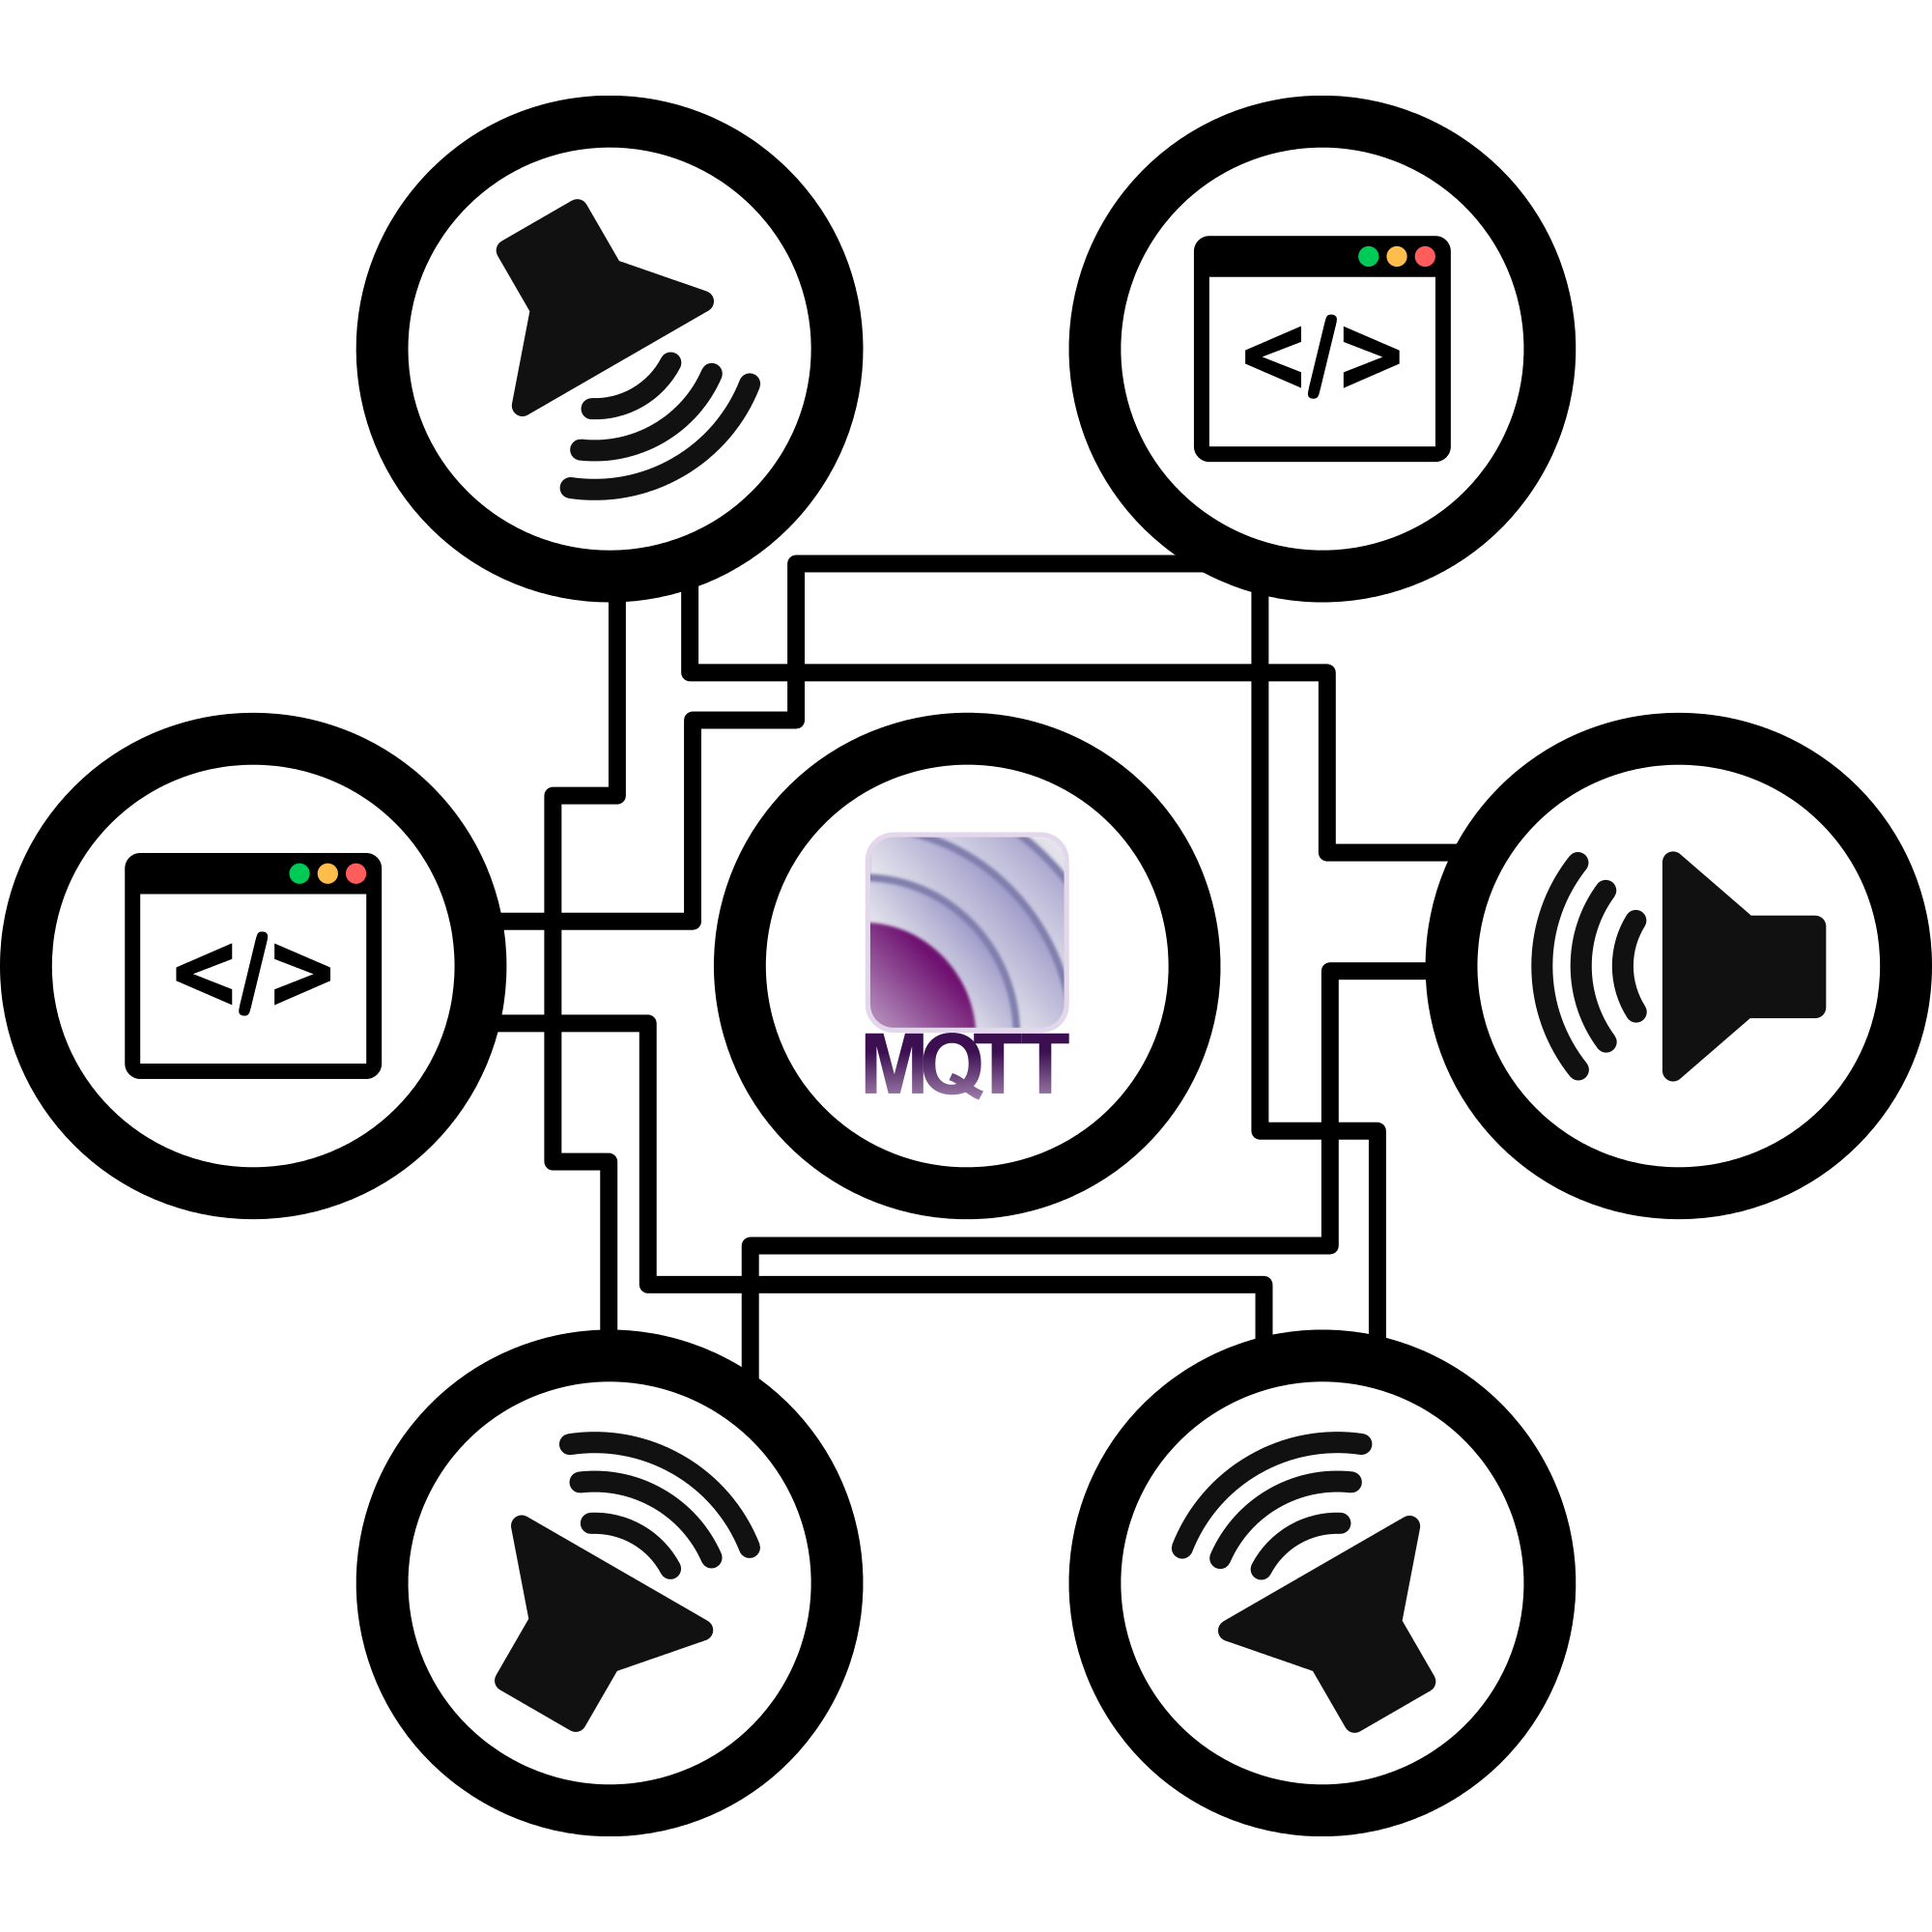
\includegraphics[height=.2\paperheight]{dynamic_network_of_speakers}
\end{figure}
